\documentclass[a4paper,UTF8,titlepage]{ctexart}
\CTEXsetup[format={\Large\bfseries}]{section}
\usepackage{amsmath}
\usepackage{caption}
\usepackage{graphicx}
\usepackage{float}
%\usepackage{epsfig}
%\usepackage{subfig}
\usepackage{subfigure}
%\usepackage{subcaption}
\usepackage{diagbox}
\def\pgfsysdriver{pgfsys-dvipdfmx.def}
\usepackage{tikz}
\usepackage{hyperref}
\pagestyle{plain}

\hypersetup{colorlinks=true,linkcolor=black}
\begin{document}
\title{带间断系数的弹性问题}
\date{\today}
\maketitle

\renewcommand{\abstractname}{\vspace{-2em}\large\bf 摘要}
\begin{abstract}
	客观世界下的很多能接触到的材料都不仅仅是单一的材料构成,往往由不同种材料复合而来。其中不同材料复合而来的物理现象所构成的数学模型即为界面问题。材料之间的间断面称之为界面, 且在上述模型中, 模型的解通常受间断系数的影响需要满足某种跳跃条件, 即服从某种意义上的守恒律. 界面问题在足够光滑的界面条件下,其解也会在此区域上光滑. 但是由于解在界面上的跳跃, 导致使用一般的数值解法很难在解的整体光滑性较差的情况下还能有比较理想的逼近效果和逼近精度.本文采用非协调有限元对二维情况下弹性界面问题进行求解  \\
	\noindent{关键字:\textbf{弹性界面问题};\textbf{非协调有限元};     \textbf{locking-free}}
\end{abstract}
\thispagestyle{empty}

\newpage
\tableofcontents

\newpage

\section{引言}

\subsection{研究背景}

具有间断系数的方程成为交界面问题。这类问题起源于许多应用领域,例如2种不同材料或者相同材料在不同状态下物理机制的研究 \textsuperscript{\cite{邵文婷2017求解一类交界面问题的模态基函数谱元法数值实验}}、声音在水中的传递、海市蜃楼现象等,同时在数值模拟等场景中也有者大量的界面问题。

平面弹性力学方程组是弹性力学中最基础、最常见的模型。当研究的弹性体形状和受力具有一定特点时,通过适当的简化处理,就可以归结为平面弹性问题 \textsuperscript{\cite{王兆清2018不可压缩平面问题的位移}}。
对于各向同性均匀介质的平面弹性问题,当材料的Lam$\acute{e}$常数$\lambda \to \infty$时,即对于几乎不可压介质,通常低阶的协调有限元解,往往不再收敛到原问题的解,或者达不到最优收敛阶,这就是闭锁现象\textsuperscript{\cite{陈绍春2007平面弹性的一个新的}}。

为了消除(近)不可压缩弹性问题中遇到的锁定现象,国内外研究学者提出了多种有效的数值分析方法。根据型函数建立过程中是否需要网格剖分,这些数值方法可以分为两类:一类是有网格方法,这其中包括
高阶有限元法\textsuperscript{\cite{peet2014legendre}}、
混合有限元法\textsuperscript{\cite{masud2011variational}}、
增强有限元法\textsuperscript{\cite{auricchio2005analysis}}和
不连续Galerkin法\textsuperscript{\cite{hansbo2003discontinuous}}等;
另一类是无网格方法,无网格方法又可分为弱形式无网格法和强形式的无网格方法\textsuperscript{\cite{王兆清2018不可压缩平面问题的位移}}。

本文将通过数值实验的方法,考察对于具有间断系数的平面弹性问题,使用C-R元是否仍可以解除闭锁现象。

\subsection{国内外研究现状}

1943年,R.W.Courant首次提出有限元法的核心思想。1956年,R.W.Clough等四位教授与工程师在科技期刊上发表一篇计算飞机机翼强度的论文,且把这种解法称之为刚性法(Stiffness),是有限元法在工程学界上的开端。1960年,R.W.Clough教授发表的平面弹性论文中,“有限元法”这个名称被首次使用,同时也将有限元法扩展到土木工程上。1963年,Richard MacNeal博士与Robert Schwendler联手创办了MSC公司,并开发了第一个软件程序,名为SADSAM,即数字仿真模拟结构分析,标志着有限元方法(FEA)由理论向程序的转变,1964-1965年,O.C.Zienkiewicz等人发表关于利用极小位能原理和虚功原理,以新的思路推导出有限元法。

我国有限元发展之路中较为著名的有:冯康(有限单元法理论),钱令希(余能定理),钱伟长(广义变分原理)等等。但是受限与当时的国际和国内环境,我国的学者在有限元方法上的进一步研究困难重重,很难跟上国际潮流,遗憾的被国外拉开距离。在之后的十年,伴随者国内有限元软件和有限元方法理论的诞生和发展,大型工程也逐渐使用有限元方法来计算,如水利、机械等多个领域,并且也都取得了不错的效果。上世纪90年代,国外的有限元软件大批量地涌入国内市场,涉及到各个领域。国外的学者专家也都进入各大学、工厂与企业进行宣传他们所掌握的技术和使用技巧,导致国内有限元发展更加困难。管理部门对有限元软件的认知上产生了偏差,对此失去了必要的支持,核心技术掌握在国外,所以至上世纪最后十几年里,国内自主技术创新的进度十分缓慢。但是进入21世纪后,国内自主知识产权的软件逐渐市场化,获得了一定的发展,同时也获得了国家对有限元技术的关注,逐渐走出低迷状态,有限元技术也不再仅仅停留在高校和企业中。

\section{有限元理论}

\subsection{Sobolev空间}

假定 G 是有界平面区域,其边界 $\Gamma$ 是按段光滑的简单闭曲线,$\overline{G} = G \cup \Gamma$ 是 G 的闭包。对于 $\overline{G}$ 上的任一函数 u(x,y),称集合{(x,y) | u(x,y) $\ne$ 0, (x,y) $\in \overline{G}$} 的闭包为 u 的支集。如果 u 的支集 $\in$ G 内,则说 u 于 G 具有紧致支集。具有紧致支集的函数必在边界 $\Gamma$ 的某一邻域内恒等于零\textsuperscript{\cite{李荣华2007偏微分方程数值解}}。

用 $C_0^{\infty} $ 表示 G 上无穷次可微并具有紧致支集的函数类,$L^2(G)$ 是定义在 G 上平方可积的可测函数空间,其内积和范数分别为
$$
\begin{matrix}
	(f,g) = \int_G fg dxdy \\ 
	||f || = \sqrt{(f,f)} = (\int_G |f|^2 dxdy)^{\frac{1}{2}}
\end{matrix}
$$

对 $f \in L^2(G)$,如果存在g,h $\in L^2(G)$,使等式
$$
\begin{matrix}
	\int_G g \varphi dxdy = - \int_g f \frac{\partial \varphi}{\partial x} dxdy \\
	\int_G h \varphi dxdy = - \int_G f \frac{\partial \varphi}{\partial y} dxdy
\end{matrix}
$$ 

对任意的 $\varphi \in C_0^{\infty}$ 成立,则说 f 对 x 的一阶广义导数 g 和对 y 的一阶导数 h,记作
$$
\begin{matrix}
	f_x = \frac{\partial f}{\partial x} = g \\
	f_y = \frac{\partial f}{\partial y} = y
\end{matrix}
$$

定义 
$$
	H^1(G) = \{f(x,y) | f, f_x, f_y \in L^2(G) \}
$$
其中 $f_x, f_y $ 是 f 的广义导数。与 $H^1(G)$ 引入内积
$$
	(f,g)_1 = \int_G [fg + f_x g_x + f_y g_y] dxdy
$$
和范数
$$
	||f||_1 = \sqrt{(f,f)} = (\int_G [|f|^2 + |f_x|^2 + |f_y|^2] dxdy )^{\frac{1}{2}}
$$

则 $H^1$ 是 Hilbert 空间,称之为 Sobolev 空间。
\subsection{误差估计}

假设$\Omega$是一个凸多边形区域,并且$\Gamma_1$ or $\Gamma_2$中任意一个为空。对于纯位移问题($\Gamma_2=\emptyset$),只考虑齐次边界条件。
\par
令$T^h$ 是$\Omega$ 三角划分的一个非退化族。对于纯位移问题($\Gamma_2=\emptyset$),我们使用有限元空间
% \begin{equation}\label{equ1} (\ref{newton})引用
	%	V_h := \{ \nu \in H^1(\Omega) : \nu |_{\emph{T}} \mbox{为线性函数}, \forall \emph{T} \in \emph{T}^h \}
	% \end{equation}
$$
V_h := \{ \nu \in H^1(\Omega) : \nu |_{T} , \forall T \in T^h \},
$$
并且对于纯牵引力问题($\Gamma_1 = \emptyset$),使用
% \begin{equation}\label{equ2}
	%	V_h :=
	%\end{equation}
	$$
	V_h := \{ \nu \in H^1(\Omega) : \nu |_{T} , \forall T \in T^h \},
	$$
%	\\ \\
%	根据第二章和第四章的理论我们得到以下定理。
	\textbf{Theorem\textsuperscript{\cite{brenner2008mathematical}}.} 令 $u \in H^2(\Omega) \cap H^1(\Omega)$ 满足纯位移问题,并且$u_h \in V_h$ 满足
	$$
	a(u_h, \nu) = \int_{\Omega} f \cdot \nu dx \quad \forall \nu \in V_h.
	$$
	\\
	则存在一个正常数$C_{(\mu, \lambda)}$ 使得
	$$
	\quad \quad \quad
	\| u - u_h \|_{H^1(\Omega)} \le C_{(\mu, \lambda)} h \| u \|_{H^2(\Omega)}.
	$$
	\textbf{Theorem\textsuperscript{\cite{brenner2008mathematical}}.} 令 $u \in H^2(\Omega)$ 满足纯牵引力问题。令 $u_h \in V_h$ 满足
	$$
	a(u_h,\nu) = \int_{\Omega} f \cdot \nu dx + \int_{\Gamma} t \cdot \nu ds \quad \forall \nu \in V_h.
	$$ 
	\\
	则存在一个正常数$C_{(\mu, \lambda)}$ 使得\textsuperscript{\cite{brenner2008mathematical}}
	$$
	\| u - u_h \|_{H^1(\Omega)} \le C_{(\mu, \lambda)} h \| u \|_{H^2(\Omega)}.
	$$
%	对于一般情况 $ \emptyset \ne \Gamma_1 \ne \partial \Omega $ 下的收敛定理,查看练习 11.x.25. 
%	\\

\subsection{闭锁现象}

	对于固定的 $\mu$ 和 $\lambda$,以上定理给出了弹性问题令人满意近似的有限元近似。但是这些有限元方法的性能随着 $\lambda$ 趋向于 $\infty$ 而变差。这就是所谓的锁定现象\textsuperscript{\cite{brenner2008mathematical}}。
	\par 
	令 $\Omega = (0,1) \times (0,1)$. 考虑 $\mu = 1$ 时的纯位移边值问题:
	$$
	\begin{matrix}
		div \{ 2 \epsilon (u^{\lambda}) + \lambda tr (\epsilon (u^{\lambda})) \delta \} = f \quad in \quad \Omega \\ \quad \quad \quad \quad \quad 
		u^{\lambda}|_{\partial \Omega} =  0.
	\end{matrix}
	$$
	注意给定的 f ,当 $\lambda \to \infty$,$\| div u^{\lambda} \|_{H^1(\Omega)} \to 0$.换句话说,我们正在处理一种几乎不可能压缩的弹性材料。为了强调对 $\lambda$ 的依赖,将应力张量 $\sigma_{\lambda}(\nu)$ 和 变分形式 $a_{\lambda}(\nu,\omega)$ 表示为
	$$
	\begin{matrix}
		\sigma_{\lambda}(\nu) = 2 \epsilon(\nu) + \lambda tr (\epsilon(\nu)) \delta \\
		a_{\lambda}(\nu,\omega) = \int_{\Omega} \{ 2 \epsilon(\nu) : \epsilon(\omega) + \lambda div \nu div \omega \} dx.
	\end{matrix}
	$$
	
	令 $T^h$ 为 $\Omega $ (图 1) 的一个规则三角剖分。对于每一个 $u \in H^2(\Omega) \cap H_0^1(\Omega)$,定义 $u_h^{\lambda} \in V_h$ 为以下方程组的特解
	$$
	\begin{matrix}
		a_{\lambda}(u_h^{\lambda},\nu) = \int_{\Omega} 
		[ -div \sigma_{\lambda}(u) ] \cdot \nu dx \quad \forall \nu \in V_h. \\
		V_h := \{ \nu \in H^1(\Omega) : \nu |_{T}, \forall T \in T^h \}
	\end{matrix}
	$$
	
%	\begin{figure}[hbt]
%		\centering
%		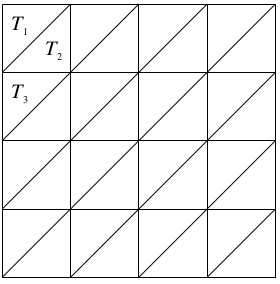
\includegraphics{../image/Fig.11.1.png}
%		\caption{单位正方形的规则三角剖分}
%	\end{figure}

\begin{figure}[ht]
	\centering
	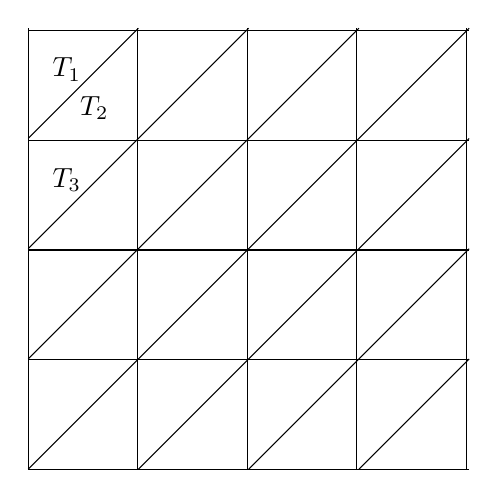
\begin{tikzpicture}[scale=0.7]
		\draw [step=56.56pt] (0,8) grid (8,0);
		
		\draw (0,6) -- (2,8);
		\draw (0,4) -- (4,8);
		\draw (0,2) -- (6,8);
		\draw (0,0) -- (8,8);
		\draw (2,0) -- (8,6);
		\draw (4,0) -- (8,4);
		\draw (6,0) -- (8,2); 
		
		\node at(0.7,7.25) {$T_1$};
		\node at(1.2,6.55) {$T_2$};
		\node at(0.7,5.25) {$T_3$};
	\end{tikzpicture}
	\caption{}
\end{figure}
	
	定义 $L_{\lambda,h}$ 为
	$$
	L_{\lambda,h} := sup \{ \frac{|u-u_h^{\lambda}|_{H^1(\Omega)}}{\| div \sigma_{\lambda}(u) \|_{L^2(\Omega)}} : 0 \ne u \in H^2(\Omega) \cap H^1(\Omega) \}.
	$$
	\\ 
	则存在一个与 h 无关的正常数 C 使得\textsuperscript{\cite{brenner2008mathematical}}
	\begin{equation}
	\lim\limits_{\lambda \to \infty} \inf L_{\lambda,h} \ge C . \label{ab}
	\end{equation}
	式 $\eqref{ab}$ 意味着:无论 h 取多小,只要 $\lambda$ 足够大,我们都能找到 $u \in H^2(\Omega) \cap H^1(\Omega)$ 使得相对误差$ |u-u_h|_{H^1(\Omega)} / \| div \sigma_{\lambda}(u) \|_{L^2(\Omega)} $ 以一个与 h 无关的常数为下界。换句话说,有限元方法的性能将会随着 $\lambda$ 变大而变坏。
	\par
	\iffalse
	为证明式 $\eqref{ab}$,首先观察到
	$$
	\{ \nu \in V_h : div \nu = 0 \} = \{ 0 \}
	$$
	因此,映射 $\nu \to div \nu$ 是有限维空间 $V_h$ 到 $L^2(\Omega)$ 的一个一对一映射,并且存在一个正常数 $C_1(h)$ 使得
	$$
	\| \nu \|_{H^1(\Omega)} \le C_1(h) \| div \nu \|_{L^2(\Omega)} \quad \forall \nu \in V_h.
	$$
	令 $\psi$ 是 $\overline{\Omega}$ 上的无穷次可微函数,使得在 $\Omega$ 的边界上 $curl \psi = 0$ 且 $\| \epsilon(curl \psi) \|_{L^2(\Omega)} = 1$。令 $u := curl \psi$。则 $u \in H^2(\Omega) \cap H^1(\Omega)$,并有
	\begin{align}	
	div u = 0, \label{a2} \\
	\| \epsilon(u) \|_{L^2(\Omega)} = 1, \label{a3}\\
	\sigma_{\lambda}(u) = 2 \epsilon(u).  \label{a4}
	\end{align}
	根据 $\eqref{a2}$, $\eqref{a4}$ 和分步积分得
	\begin{align}
	- \int_{\Omega} div \epsilon(u) \cdot u dx = \int_{\Omega} \epsilon(u) : \epsilon(u) dx = 1. \label{a5}
	\end{align}
	根据 $\eqref{a4}$, $\eqref{a5}$ 推断
	$$
	\quad \quad \quad \quad \quad \quad \quad
	\lim\limits_{\lambda \to \infty} div \sigma_{\lambda}(u) = 2 div \epsilon(u) \ne 0. 
	$$
	由 (2.5.10) 得,
	$$
	a_{\lambda}(u-u_h^{\lambda}, u-u_h^{\lambda}) = \min\limits_{\nu \in V_h} a_{\lambda}(u-\nu,u-\nu) \le a_{\lambda}(u,u).
	$$
	由 $\eqref{a2}$ 和 $\eqref{a3}$,得到
	$$
	a_{\lambda}(u,u) = 2.
	$$
	因此,对于 $\lambda$ 足够大时有
	\begin{align} 
	a_{\lambda} (u-u_h^{\lambda}, u-u_h^{\lambda}) \le 2. \label{a6}
	\end{align}
	由 $\eqref{a2}$ 和 $\eqref{a6}$ 得
	\\
	$$
	\begin{matrix}
		\sqrt{\lambda} \| div u_h^{\lambda} \|_{L^2(\Omega)} = \sqrt{\lambda} \| div(u-u_h^{\lambda}) \|_{L^2(\Omega)} \\ 
		\quad \quad \quad \quad \quad \quad \quad
		\le \sqrt{a_{\lambda}(u-u_h^{\lambda}, u-u_h^{\lambda})} \\
		\le \sqrt{2}	
	\end{matrix}
	$$
	\\
	对足够大的 $\lambda$ 有
	$$
	\lim\limits_{\lambda \to \infty} \| div u_h^{\lambda} \|_{L^2(\Omega)} = 0.
	$$
	\\
	由式 $\eqref{ab}$ 有
	$$
	\lim\limits_{\lambda \to \infty} \| u_h^{\lambda} \|_{H^1(\Omega)} = 0.
	$$
	最后,得到 %(cf.exercise 11.x.16)
	$$ 
	\begin{matrix}
		\lim\limits_{\lambda \to \infty}\inf L_{\lambda,h} \ge \lim\limits_{\lambda \to \infty}\inf \frac{|u-u_h^{\lambda}|_{H^1(\Omega)}}{\| div \sigma_{\lambda}(u) \|_{L^2(\Omega)}} \\
		\quad \quad \quad \quad
		= \frac{|u|_{H^1(\Omega)}}{\| div \sigma(u) \|_{L^2(\Omega)}} > 0.
	\end{matrix}
	$$
	\fi

\subsection{剖分与基函数}

\subsubsection{剖分}

对正方形区域 $\Omega$ 按图2方式剖分,并对节点和单元进行编号,各节点坐标为$(x_i,y_i)$, i=0, ... , n,

%\begin{figure}[hbt]
%	\centering
%	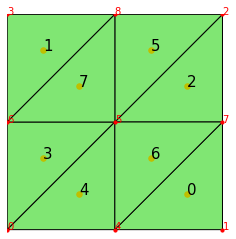
\includegraphics[height=4cm,width=4cm]{../image/subdivsion.png}
%	\caption{}
%\end{figure}

\begin{figure}[h]
	\centering
	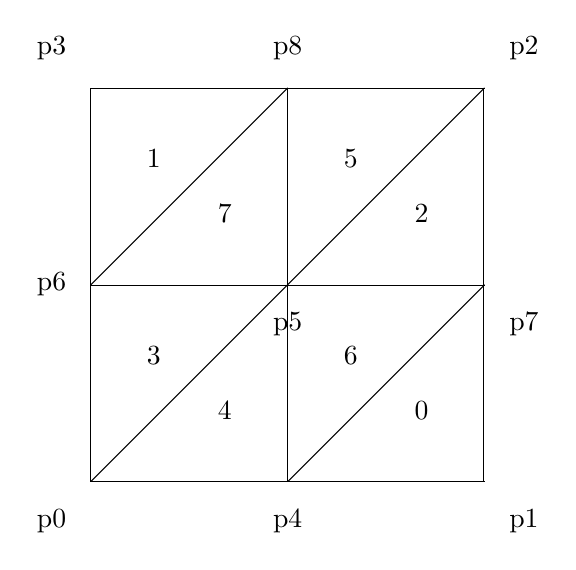
\begin{tikzpicture}
		\draw [step=71pt] (0,5) grid (5,0);
		
		\draw (0,0)--(5,5);
		\draw (0,2.5)--(2.5,5);
		\draw (2.5,0)--(5,2.5);
		
		\node at(-0.5,-0.5) {p0};
		\node at(2.5,-0.5)  {p4};
		\node at(5.5,-0.5)  {p1};
		\node at(-0.5,2.5)  {p6};
		\node at(2.5,2)     {p5};
		\node at(5.5,2)     {p7};
		\node at(-0.5,5.5)  {p3};
		\node at(2.5,5.5)   {p8};
		\node at(5.5,5.5)   {p2};
		
		\node at(0.8,1.6) {3};
		\node at(1.7,0.9) {4};
		\node at(3.3,1.6) {6};
		\node at(4.2,0.9) {0};
		\node at(0.8,4.1) {1};
		\node at(1.7,3.4) {7};
		\node at(3.3,4.1) {5};
		\node at(4.2,3.4) {2};
	\end{tikzpicture}
	\caption{划分}
	\label{1}
\end{figure}

\iffalse
设基函数为 
$$ 
(\varphi_0,0)^t, (0,\varphi_0)^t, (\varphi_1,0)^t, (0,\varphi_1)^t, ... , (\varphi_n,0)^t, (0,\varphi_n)^t 
$$

$\varphi_i$ 为线性元,以下得到其在各单元上表达式。 
\fi

\subsubsection{线性元}

如图3,设 $ \bigtriangleup(p_0,p_1,p_2) $ 是以 $p_0,p_1,p_2$ 为顶点的任意三角型元,面积为S。在 $ \bigtriangleup (p_0,p_1,p_2) $ 内任取一点p,坐标为$(x,y)$。过p点作与三个顶点的连线,将 $ \bigtriangleup(p_0,p_1,p_2) $ 分成三个三角形: $ \bigtriangleup(p_1,p_2,p), \bigtriangleup(p_0,p,p_2), \bigtriangleup(p_0,p_1,p) $,其面积分别为$S_0,S_1,S_2$ \textsuperscript{\cite{李荣华2007偏微分方程数值解}}

%\begin{figure}[hbt]
%	\centering
%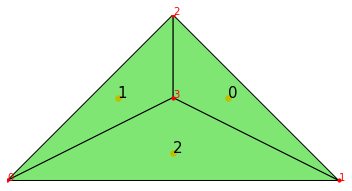
\includegraphics[height=3cm,width=4cm]{../image/TriangleElement.png}
%	\caption{}
%	\label{SampleOfDatasets}
%\end{figure}

\begin{figure}[h]
	\centering
	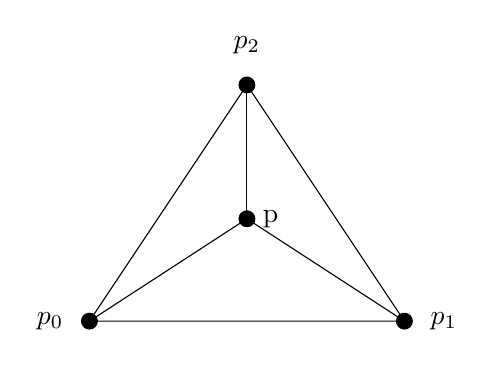
\begin{tikzpicture}
		\draw (3,0)--(7,0)--(5,3)--cycle;
		\draw (3,0)--(5,1.3)--(7,0);
		\draw (5,1.3)--(5,3);
		\filldraw (3,0)   circle(.1)
		(7,0) circle(.1)
		(5,3) circle(.1)
		(5,1.3) circle(.1);
		\node at(2.5,0)  {$p_0$};
		\node at(7.5,0)   {$p_1$};
		\node at(5,3.5)   {$p_2$};
		\node at(5.3,1.3) {p};
	\end{tikzpicture}
	\caption{}
	\label{1}
\end{figure}

显然$S_0 + S_1 + S_2 = S$,令
$$
L_0 = \frac{S_0}{S}, \quad L_1 = \frac{S_1}{S}, \quad L_2 = \frac{S_2}{S}
$$
\par
%称$(L_0,L_1,L_2)$位$P_3$的面积坐标,其中
%$$
%	\begin{cases}
	%		2S = \left| \begin{matrix}
		%				1 & x_0 & y_0 \\
		%				1 & x_1 & y_1 \\
		%				1 & x_2 & y_2
		%			 \end{matrix} \right| ,
	%		 \quad
	%		 2S_0 = \left| \begin{matrix}
		%		 			1 & x   & y   \\
		%		 			1 & x_1 & y_1 \\
		%		 			1 & x_2 & y_2
		%		 \end{matrix} \right| 
	%		 \\
	%		2S_1 = \left| \begin{matrix}
		%					1 & x_0 & y_0 \\
		%					1 & x   & y   \\
		%					1 & x_2 & y_2
		%			   \end{matrix} \right|,
	%		\quad
	%		2S_2 = \left| \begin{matrix}
		%					1 & x_0 & y_0 \\
		%					1 & x_1 & y_1 \\
		%					1 & x   & y
		%			   \end{matrix} \right|
	%	\end{cases}
%$$

%由此可得面积坐标和直角坐标的转化关系
%$$
%\begin{cases}
%	x = x_0 L_0 + x_1 L_1 + x_2 L_2 \\
%	y = y_0 L_0 + y_1 L_1 + x_2 L_2
%\end{cases}
%$$
$$
\begin{cases}
	L_0 = \frac{1}{2S} [(x_2 y_3 - x_3 y_2) + (y_2 - y_3) x + (x_3 - x_2) y] \\
	L_1 = \frac{1}{2S} [(x_3 y_0 - x_0 y_3) + (y_3 - y_0) x + (x_0 - x_3) y] \\
	L_2 = \frac{1}{2S} [(x_0 y_1 - x_1 y_0) + (y_0 - y_1) x + (x_1 - x_0) y]
\end{cases} 
$$

因为

$$
\begin{cases}
	L_0 = \begin{cases}
		1, \quad x = x_0, y = y_0 \\
		0, \quad x = x_1, y = y_1 \\
		0, \quad x = x_2, y = y_2
	\end{cases} \\
	L_1 = \begin{cases}
		0, \quad x = x_0, y = y_0 \\
		1, \quad x = x_1, y = y_1 \\
		0, \quad x = x_2, y = y_2
	\end{cases} \\
	L_2 = \begin{cases}
		0, \quad x = x_0, y = y_0 \\
		0, \quad x = x_1, y = y_1 \\
		1, \quad x = x_2, y = y_2
	\end{cases} \\
\end{cases}
$$

所以在此区间上 $\varphi_i = L_i$,即。

$$
\begin{cases}
	\varphi_0 = \frac{1}{2S} [(x_2 y_3 - x_3 y_2) + (y_2 - y_3) x + (x_3 - x_2) y] \\
	\varphi_1 = \frac{1}{2S} [(x_3 y_0 - x_0 y_3) + (y_3 - y_0) x + (x_0 - x_3) y] \\
	\varphi_2 = \frac{1}{2S} [(x_0 y_1 - x_1 y_0) + (y_0 - y_1) x + (x_1 - x_0) y]
\end{cases} 
$$


\subsubsection{CR元}

如图4,设三角形 $\bigtriangleup(q_0,q_1,q_2)$ 是以 $q0,q1,q2$ 为顶点的任意三角形元,$p_0,p_1,p_2$ 为其三条边的中点,其坐标分别为$(x_0.y_0),(x_1,y_1),(x_2,y_2)$。

\begin{figure}[h]
	\centering
	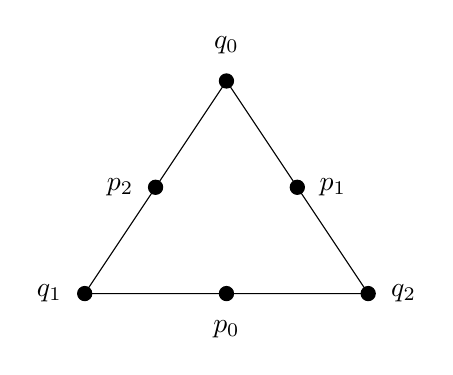
\begin{tikzpicture}[scale=0.9]
		\draw (0,0)--(4,0)--(2,3)--cycle;
		\filldraw (2,0)   circle(.1)
				  (3,1.5) circle(.1)
				  (1,1.5) circle(.1)
				  (0,0) circle(.1)
				  (4,0) circle(.1)
				  (2,3) circle(.1);
		
		\node at(2,-0.5)  {$p_0$};
		\node at(3.5,1.5) {$p_1$};
		\node at(0.5,1.5) {$p_2$};
		
		\node at(-0.5,0) {$q_1$};
		\node at(4.5,0) {$q_2$};
		\node at(2,3.5) {$q_0$};
	\end{tikzpicture}
	\caption{}
	\label{1}
\end{figure}

设三角形 $\bigtriangleup(q_0,q_1,q_2)$ 上的CR元为 $\varphi_0, \varphi_1,\varphi_2$,

$$
	\varphi_i = a_i x + b_i y + c_i, \quad i = 0,1,2
$$

$$
	\varphi_i(p_j) = \begin{cases}
		1, \quad i = j \\
		0, \quad i \ne j	
	\end{cases}, \quad i, j = 0,1,2
$$

设

$$
	A = \begin{bmatrix}
		x_0 & y_0 &1 \\
		x_1 & y_1 &1 \\
		x_2 & y_2 &1 \\
	\end{bmatrix}, \quad 
	c_i = (a_i,b_i,c_i)^t , \quad
	f = (x,y,1)^t
$$

则

$$
	A c_i = e_i, \quad i = 0,1,2
$$

所以

$$
	c_i = A^{-1} e_i
$$

$$
	\varphi_i = A^{-1} e_i f, \quad i = 0,1,2
$$ 

\iffalse
$$
\begin{cases}
	\begin{cases}
		\varphi_0(p_0) = a_0 x_0 + b_0 y_0 + c_0 = 1 \\
		\varphi_0(p_1) = a_0 x_1 + b_0 y_1 + c_0 = 0 \\
		\varphi_0(p_2) = a_0 x_2 + b_0 y_2 + c_0 = 0
	\end{cases} \\
	\begin{cases}
		\varphi_1(p_0) = a_1 x_0 + b_1 y_0 + c_1 = 0 \\
		\varphi_1(p_1) = a_1 x_1 + b_1 y_1 + c_1 = 1 \\
		\varphi_1(p_2) = a_1 x_2 + b_1 y_2 + c_1 = 0 
	\end{cases} \\
	\begin{cases}
		\varphi_2(p_0) = a_2 x_0 + b_2 y_0 + c_2 = 0 \\
		\varphi_2(p_1) = a_2 x_1 + b_2 y_1 + c_2 = 0 \\
		\varphi_2(p_2) = a_2 x_2 + b_2 y_2 + c_2 = 1
	\end{cases}
\end{cases}
$$
\fi

\section{算例}

\subsection{弹性问题}

\subsubsection{模型}

令
$$
\begin{matrix}
	\sigma(u) = 2 \mu \epsilon(u) + \lambda tr(\epsilon(u)) \delta \\
	\epsilon(u) = \frac{1}{2} (grad u + (grad u)^t) \\
	tr(\tau) = \tau_{11} + \tau_{22} \\
	grad(u) = \begin{pmatrix}
		\frac{\partial u_1}{\partial x} & \frac{\partial u_1}{\partial y} \\
		\frac{\partial u_2}{\partial x} &
		\frac{\partial u_2}{\partial y}
	\end{pmatrix} \\
	\delta = \begin{pmatrix}
		1 & 0 \\
		0 & 1
	\end{pmatrix} \\
	div u = \frac{\partial u_1}{\partial x} + \frac{\partial u_2}{\partial y} \\
	div \tau = \begin{pmatrix}
		\frac{\partial \tau_{11}}{\partial x} + \frac{\partial \tau_{12}}{\partial y} \\
		\frac{\partial \tau_{12}}{\partial x} + \frac{\partial \tau_{22}}{\partial 
		y}
	\end{pmatrix}
\end{matrix}
$$

考察模型
$$
\begin{matrix}
	-div \sigma(u) = f \quad \in \Omega  \\
	u |_{\Gamma} = 0
	%(\sigma(u) \nu) |_{\Gamma2} = t
\end{matrix}
$$ 
\par
其中$ u = (u_1,u_2)^t $ 为求解向量,$ f = (f_1,f_2)^t $为右端向量,$ \Omega = [0,1] \times [0,1] $
$$
\begin{matrix}
	u_1 = (x - 1)(y - 1) y sin(x) 
	\\
	u_2 = (x - 1)(y - 1) x sin(y) 
	\\
	f_1 = -((2 \mu + \lambda) y (y - 1) (2 cos(x) - (x - 1) sin(x)) \\
	+ (\mu + \lambda) (2 x - 1) (sin(y) + (y - 1) cos(y)) \\
	+ 2 \mu (x - 1) sin(x)) 
	\\
	f_2 = -((2 \mu + \lambda) x (x - 1) (2 cos(y) - (y - 1) sin(y)) \\
	+ (\mu + \lambda) (2 y - 1) (sin(x) + (x - 1) cos(x)) \\ 
	+ 2 \mu (y - 1) sin(y))
\end{matrix}
$$

\subsubsection{变分}

设 $\nu = (\nu_1,\nu_2)^t, \quad \nu_1, \nu_2 \in C_0^{\infty}(\Omega)$,方程两边同乘 $\nu$ 并积分得
$$
-\int_{\Omega} div \sigma(u) \nu dxdy = \int_{\Omega} f \nu dxdy
$$

由
$$
\begin{matrix}
	f div a = div(fa) - a : grad f \\
	\int_{\Omega} div a dV = \int_{\partial \Omega} a dS
\end{matrix}
$$

得
\par \quad \quad
$-\int_{\Omega} div \sigma(u) \nu dxdy$
$$ 
\quad \quad
\begin{matrix}
	\begin{aligned}
		&= -\int_{\Omega} div(\sigma(u) \nu) dxdy - \int_{\Omega} \sigma(u) : grad \nu dxdy \\
		&= -\int_{\Gamma} \sigma(u) \nu dxdy + \int_{\Omega} \sigma(u) : grad \nu dxdy \\
		&= \int_{\Omega} \sigma(u) : grad \nu dxdy \\
		&= \int_{\Omega} 2 \mu \epsilon(u) : grad \nu + \lambda div u div \nu dxdy  \\
		&= \mu \int_{\Omega} grad u : grad \nu dxdy + (\mu +\lambda) \int_{\Omega} div u div \nu  dxdy
	\end{aligned}
\end{matrix}
$$

所以
$$
\mu \int_{\Omega} grad u : grad \nu dxdy + (\mu +\lambda) \int_{\Omega} div u div \nu  dxdy = \int_{\Omega} f \nu dxdy
$$

该问题的变分问题为,求$u \in H^1(\Omega)$ 使得 $u |_{\Gamma_1} = g$,并且
$$
	a(u,\nu) = \int_{\Omega} f \cdot \nu dxdy \quad \forall \nu \in V
$$ 
\par
其中
$$
	\begin{matrix}
		\begin{aligned}
			a(u,\nu) :&= \mu \int_{\Omega} grad u : grad \nu dxdy + (\mu +\lambda) \int_{\Omega} div u div \nu  dxdy \\  
			
			V :&= \{ \nu \in H^1(\Omega) \quad | \quad \nu |_{\Gamma} = 0 \}
		\end{aligned}
	\end{matrix}
$$

%证其与原问题的等价性

%\begin{enumerate}
%	\item 若 u 为原问题的解 \\

	
%	\item 若 u 为变分问题的解 \\
%	由
%	\par \quad \quad
%	$\int_{\Omega} \sigma(u) : grad \nu dxdy$
%	$$
%	\quad \quad
%	\begin{matrix}
%		\begin{aligned}
%			&= -\int_{\Gamma} \sigma(u) \nu dxdy + \int_{\Omega} \sigma(u) : grad %\nu dxdy \\
%			&= -\int_{\Omega} div \sigma(u) \nu dxdy
%		\end{aligned}
%	\end{matrix} 
%	$$
%
%	得
%	$$
%		-\int_{\Omega} div \sigma(u) \nu dxdy = \int_{\Omega} f \nu dxdy
%	$$
%	
%	由变分法基本引理得
%	$$
%		-div \sigma(u) = f
%	$$
%	
%\end{enumerate}

\subsubsection{刚度矩阵}

设 $\varphi_{xi} = (\varphi_i, 0)^t, \varphi_{yi} = (0,\varphi_i)^t$,i = 0, ... , n 为试探函数空间$U_h$的基函数,则任一 $u_h \in U_h$ 可表成
$$
	u_h = \sum\limits_{i=1}^n u^{i}_1 \varphi_{xi} + \sum\limits_{i=1}^n u^{i}_2 \varphi_{yi}, \quad u^i = u_h(x_i,y_i)
$$ 
\\ 
令 $\phi_{2i} = \varphi_{xi}$ ,$\phi_{2i+1} = \varphi_{yi}$ , $c_{2i} = u^i_1$ , $c_{2i+1} = u^i_2$
带入变分形式得
$$
	\sum\limits_{j=0}^{2n+1} a(\phi_j, \phi_i) c_i = (f,\phi_i) \quad i=0, ... ,2n+1
$$

矩阵形式为
$$
\begin{matrix}
	A c = F \\
	A = (a(\phi_i, \phi_j))_{(2n+1) \times (2n+1)} \\
	F = ((f,\phi_i))_{(2n+1) \times 1} \\
	c = (c_i)_{(2n+1) \times 1}
\end{matrix}
$$

%\subsection{单元刚度矩阵}
%
%在第m个单元cell=$\bigtriangleup(i,j,k)$上,单元刚度矩阵和单元载荷向量为
%$$
%\begin{matrix}
%	A^{(m)} = (\int_{cell} (2 \mu \epsilon(\phi_{i_1}) : \epsilon(\phi_{j_1}) + %\lambda div \phi_{i_1} div \phi_{j_1}))_{3 \times 3} \\
%	F^{(m)} = (\int_{cell} f \cdot \phi_{i_1})_{3 \times 1} \\
%	i_1, j_1 = i, j, k
%\end{matrix} 
%$$
%
%将$A^{(m)}$扩展成$n \times n$矩阵,行列为i,j,k的九个元素即为$A^{(m)}$的九个元素,并以同样的方式将$F^{(m)}$扩展成$n \times 1$向量,则
%$$
%\begin{matrix} 
%	A = \sum\limits_{m=0}^n A^{(m)} \\
%	F = \sum\limits_{m=0}^n F^{(m)}
%\end{matrix}
%$$

\subsubsection{边界条件}

模型为齐次边界条件,若$(x_i,y_i)$为边界点,则 A 第 2i 行第 2i 列,第 2i+1 行第 2i+1 列元素为1,其他元素及  F(2i),F(2i+1) 都为0。

%\vfill \newpage

%\bibliographystyle{unsrt}
%\bibliography{interface_problem}

\subsubsection{实验结果}

通过数值实验得到,当 $\mu = 1, \lambda = 1, 1e1, ..., 1e5$ 时的误差如下表

\begin{table}[h]
	\centering
	\caption{线性元误差}
	\scalebox{0.8}{
	\begin{tabular}{|c|c|c|c|c|c|} \hline
		\diagbox{$\lambda$}{h} &1.0 &0.5 &0.25 &0.125 &0.0625 \\ \hline
		1 &0.0 &5.3881e-5 &1.1197e-4 &3.9125e-5 &1.0772e-5 \\ \hline
		10 &0.0 &1.1963e-2 &2.6789e-3 &6.4168e-4 &1.6060e-4  \\ \hline
		100 &0.0 &1.8830e-2 &4.7420e-3 &1.2635e-3 &3.5042e-4  \\ \hline
		1e3 &0.0 &1.9855e-2 &5.2306e-3 &1.6399e-3 &6.7184e-4  \\ \hline
		1e4 &0.0 &1.9963e-2 &5.2878e-3 &1.7076e-3 &6.6349e-4  \\ \hline
		1e5 &0.0 &1.9974e-2 &5.2936e-3 &1.7150e-3 &8.2476e-4 \\ \hline
	\end{tabular}}
\end{table}

\iffalse
\begin{figure}[h]
	\centering
	\subfigure[$\lambda$=1]{
		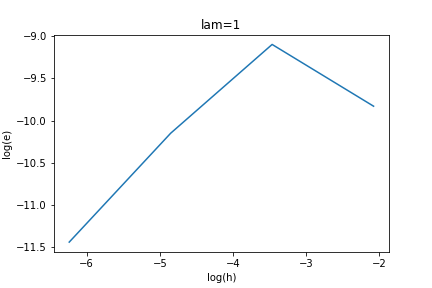
\includegraphics[height=2cm,width=3cm]{../image/Fem/elasticityFemLam_1.png}
		\label{1}}	
	\subfigure[$\lambda$=10]{
		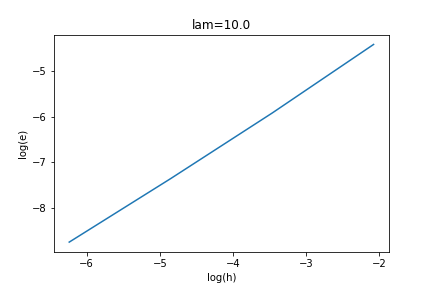
\includegraphics[height=2cm,width=3cm]{../image/Fem/elasticityFemLam_10.0.png}
		\label{10}}
	\subfigure[$\lambda$=100]{
		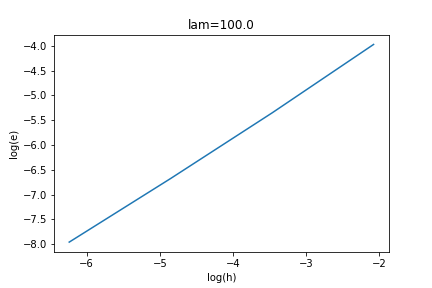
\includegraphics[height=2cm,width=3cm]{../image/Fem/elasticityFemLam_100.0.png}
		\label{100}}
	
	\subfigure[$\lambda$=1000]{
		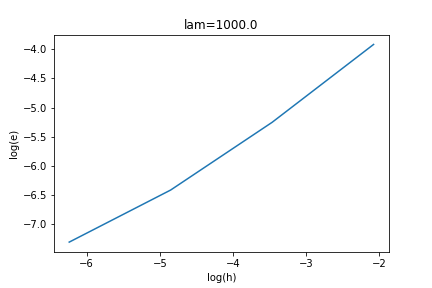
\includegraphics[height=2cm,width=3cm]{../image/Fem/elasticityFemLam_1000.0.png}
		\label{1000}}
	\subfigure[$\lambda$=10000]{
		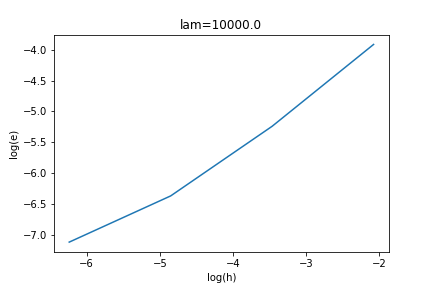
\includegraphics[height=2cm,width=3cm]{../image/Fem/elasticityFemLam_10000.0.png}
		\label{10000}}
	\subfigure[$\lambda$=100000]{
		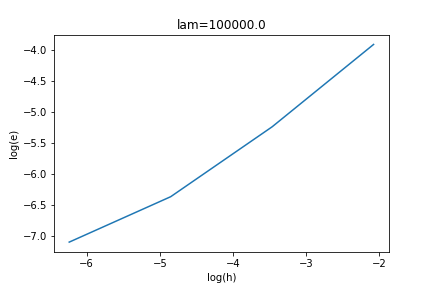
\includegraphics[height=2cm,width=3cm]{../image/Fem/elasticityFemLam_100000.0.png}
		\label{100000}}
	\caption{线性元误差}
\end{figure}
\fi

\begin{table}[h]
	\centering
	\caption{CR元误差}
	\scalebox{0.8}{
	\begin{tabular}{|c|c|c|c|c|c|} \hline
		\diagbox{$\lambda$}{h} &1.0 &0.5 &0.25 &0.125 &0.0625 \\ \hline
		1 &2.9011 &7.9878e-2 &2.0326e-2 &5.8054e-3 &1.5808e-3  \\ \hline
		10 &1.8652 &4.9859e-2 &1.2611e-2 &3.4043e-3 &9.0626e-4  \\ \hline
		100 &1.7617 &4.6901e-2 &1.1864e-2 &3.1691e-3 &8.3997e-4  \\ \hline
		1e3 &1.7513 &4.6605e-2 &1.1790e-2 &3.1457e-3 &8.3336e-4  \\ \hline
		1e4 &1.7503 &4.6577e-2 &1.1783e-2 &3.1434e-3 &8.3270e-4 \\ \hline
		1e5 &1.7502 &4.6574e-2 &1.1782e-2 &3.1431e-3  &8.3263e-4 \\ \hline
	\end{tabular}}
\end{table}

\iffalse
\begin{figure}[h]
	\centering
	\subfigure[$\lambda$=1]{
		\includegraphics[height=2cm,width=3cm]{../image/CRFem/elasticityCRfemLam_1.png}
		\label{CR1}}	
	\subfigure[$\lambda$=10]{
		\includegraphics[height=2cm,width=3cm]{../image/CRFem/elasticityCRfemLam_10.0.png}
		\label{CR10}}
	\subfigure[$\lambda$=100]{
		\includegraphics[height=2cm,width=3cm]{../image/CRFem/elasticityCRfemLam_100.0.png}
		\label{CR100}}
	
	\subfigure[$\lambda$=1000]{
		\includegraphics[height=2cm,width=3cm]{../image/CRFem/elasticityCRfemLam_1000.0.png}
		\label{CR1000}}
	\subfigure[$\lambda$=10000]{
		\includegraphics[height=2cm,width=3cm]{../image/CRFem/elasticityCRfemLam_10000.0.png}
		\label{CR10000}}
	\subfigure[$\lambda$=100000]{
		\includegraphics[height=2cm,width=3cm]{../image/CRFem/elasticityCRfemLam_100000.0.png}
		\label{CR100000}}
	\caption{CR元误差}
\end{figure}
\fi

可以看到,随着 $\lambda$ 的增大,使用线性元得到的近似解的收敛效果逐渐下降,而使用CR元的收敛速度保持不变。

\subsection{弹性界面问题}

\subsubsection{模型}

考察模型
$$
\begin{matrix}
	-div \sigma(u) = f \quad \in \Omega  \\
	u |_{\Gamma} = 0
	%(\sigma(u) \nu) |_{\Gamma2} = t
\end{matrix}
$$ 
\par
其中$ u = (u_1,u_2)^t $ 为求解向量,$ f = (f_1,f_2)^t $为右端向量,
$ 
\Omega = [0,1] \times [0,1] , \quad 
\Omega_1 = [0,0.5] \times [0,0.5] , \quad
\Omega_2 = [0.5,1] \times [0,0.5], \quad
\Omega_3 = [0,0.5] \times [0.5,1], \quad
\Omega_4 = [0.5,1] \times [0.5,1]
$ 
\par
当$(x,y) \in \Omega_1$时,$\mu = \lambda = \lambda_1$
$$
\begin{matrix}
	u_1 = (x - 1)(y - 1) y sin(x) / \lambda_1
	\\
	u_2 = (x - 1)(y - 1) x sin(y) \ \lambda_1
\end{matrix}
$$

当$(x,y) \in \Omega_2$时, $\mu = \lambda = \lambda_2$

$$
\begin{matrix}
	u_1 = (x - 1)(y - 1) y sin(x) / \lambda_2 
	\\
	u_2 = (x - 1)(y - 1) x sin(y) / \lambda_2
\end{matrix}
$$

当$(x,y) \in \Omega_3$时,$\mu = \lambda = \lambda_3$
$$
\begin{matrix}
	u_1 = (x - 1)(y - 1) y sin(x) / \lambda_3
	\\
	u_2 = (x - 1)(y - 1) x sin(y) \ \lambda_3
\end{matrix}
$$

当$(x,y) \in \Omega_4$时, $\mu = \lambda = \lambda_4$

$$
\begin{matrix}
	u_1 = (x - 1)(y - 1) y sin(x) / \lambda_4 
	\\
	u_2 = (x - 1)(y - 1) x sin(y) / \lambda_4
\end{matrix}
$$

右端向量

$$
\begin{matrix}
	f_1 = -((2 \mu + \lambda) y (y - 1) (2 cos(x) - (x - 1) sin(x)) \\
	+ (\mu + \lambda) (2 x - 1) (sin(y) + (y - 1) cos(y)) \\
	+ 2 \mu (x - 1) sin(x)) 
	\\
	f_2 = -((2 \mu + \lambda) x (x - 1) (2 cos(y) - (y - 1) sin(y)) \\
	+ (\mu + \lambda) (2 y - 1) (sin(x) + (x - 1) cos(x)) \\ 
	+ 2 \mu (y - 1) sin(y))
\end{matrix}
$$

\subsubsection{变分}

设 $\nu = (\nu_1,\nu_2)^t, \quad \nu_1, \nu_2 \in C_0^{\infty}(\Omega)$,方程两边同乘 $\nu$ 并积分得
$$
-\int_{\Omega} div \sigma(u) \nu dxdy = \int_{\Omega} f \nu dxdy
$$

由
$$
\begin{matrix}
	f div a = div(fa) - a : grad f \\
	\int_{\Omega} div a dV = \int_{\partial \Omega} a dS
\end{matrix}
$$

得
\par \quad \quad
$-\int_{\Omega} div \sigma(u) \nu dxdy$
$$ 
\quad \quad
\begin{matrix}
	\begin{aligned}
		&= -\int_{\Omega_1} div \sigma(u) \nu dxdy -\int_{\Omega_2} div \sigma(u) \nu dxdy - \int_{\Omega_3} div \sigma(u) \nu dxdy \\
		&-\int_{\Omega_4} div \sigma(u) \nu dxdy \\
		&= -\int_{\partial \Omega_1} div(\sigma(u) \nu) dxdy + \int_{\Omega_1} \sigma(u) : grad \nu dxdy -\int_{\partial \Omega_2} div(\sigma(u) \nu) dxdy \\
		&+ \int_{\Omega_2} \sigma(u) : grad \nu dxdy - \int_{\partial \Omega_3} div(\sigma(u) \nu) dxdy + \int_{\Omega_3} \sigma(u) : grad \nu dxdy \\
		&-\int_{\partial \Omega_4} div(\sigma(u) \nu) dxdy + \int_{\Omega_4} \sigma(u) : grad \nu dxdy \\
		&= -\int_{\Gamma} \sigma(u) \nu dxdy + \int_{\Omega_1} \sigma(u) : grad \nu dxdy 
		+ \int_{\Omega_2} \sigma(u) : grad \nu dxdy \\
		&+ \int_{\Omega_3} \sigma(u) : grad \nu dxdy + \int_{\Omega_4} \sigma(u) : grad \nu dxdy\\
		&= \int_{\Omega_1} \sigma(u) : grad \nu dxdy + \int_{\Omega_2} \sigma(u) : grad \nu dxdy + \int_{\Omega_3} \sigma(u) : grad \nu dxdy \\
		&+ \int_{\Omega_4} \sigma(u) : grad \nu dxdy \\
	\end{aligned}
\end{matrix}
$$
$$
\begin{matrix}
	\begin{aligned}
		&= \mu \int_{\Omega_1} grad u : grad \nu dxdy + (\mu +\lambda) \int_{\Omega_1} div u div \nu  dxdy \\
		&+ \mu \int_{\Omega_2} grad u : grad \nu dxdy + (\mu +\lambda) \int_{\Omega_2} div u div \nu  dxdy \\
		&+ \mu \int_{\Omega_3} grad u : grad \nu dxdy + (\mu +\lambda) \int_{\Omega_3} div u div \nu  dxdy \\
		&+ \mu \int_{\Omega_4} grad u : grad \nu dxdy + (\mu +\lambda) \int_{\Omega_4} div u div \nu  dxdy
	\end{aligned}
\end{matrix}
$$

所以,该问题的变分问题为,求$u \in H^1(\Omega)$ 使得 $u |_{\Gamma_1} = g$,并且
$$
a(u,\nu) = \int_{\Omega} f \cdot \nu dxdy \quad \forall \nu \in V
$$ 
\par
其中
$$
\begin{matrix}
	\begin{aligned}
		a(u,\nu) :&= \mu \int_{\Omega_1} grad u : grad \nu dxdy + (\mu +\lambda) \int_{\Omega_1} div u div \nu  dxdy \\
		&+ \mu \int_{\Omega_2} grad u : grad \nu dxdy + (\mu +\lambda) \int_{\Omega_2} div u div \nu  dxdy \\
		&+ \mu \int_{\Omega_3} grad u : grad \nu dxdy + (\mu +\lambda) \int_{\Omega_3} div u div \nu  dxdy \\
		&+ \mu \int_{\Omega_4} grad u : grad \nu dxdy + (\mu +\lambda) \int_{\Omega_4} div u div \nu  dxdy\\
		V :&= \{ \nu \in H^1(\Omega) \quad | \quad \nu |_{\Gamma} = 0 \}
	\end{aligned}
\end{matrix}
$$

\section{总结}

1

\newpage
\vfill

\bibliographystyle{unsrt}
\clearpage
\phantomsection
\addcontentsline{toc}{section}{参考文献}
\tolerance=500
\bibliography{interface_problem}

\end{document}